\documentclass[a4paper]{jarticle}
\usepackage{comment}
\usepackage{slashbox}
\usepackage[dvipdfmx]{graphicx}
\usepackage[top=20truemm,bottom=20truemm,left=20truemm,right=20truemm]{geometry}
\title{計算機工学実験A課題3レポート}
\author{学生番号 氏名}
\date{2016/11/24}
\begin{document}
\maketitle
\section{実験の総括的な目的}
QUARTUSを用いて様々な回路図をGUI上で設計し、それをコンパイルし、ALTERA上で実行し、様々な基本的な回路をシミュレートする。
\section{実験結果}
\subsection{課題1}
\subsubsection{目的}
フォルダex1-1を用意し、プロジェクトを開いて、トグルスイッチ(SW1 \textasciitilde SW17)を、残りの赤色LED(LEDR1 \textasciitilde LEDR17)に接続したものと、押しボタンスイッチ(KEY0 \textasciitilde KEY3)を、緑色LED(LEDG0 \textasciitilde LEDG3)に接続した回路を作成し、コンパイル・動作させる。
\subsubsection{道のり}
\begin{center}
	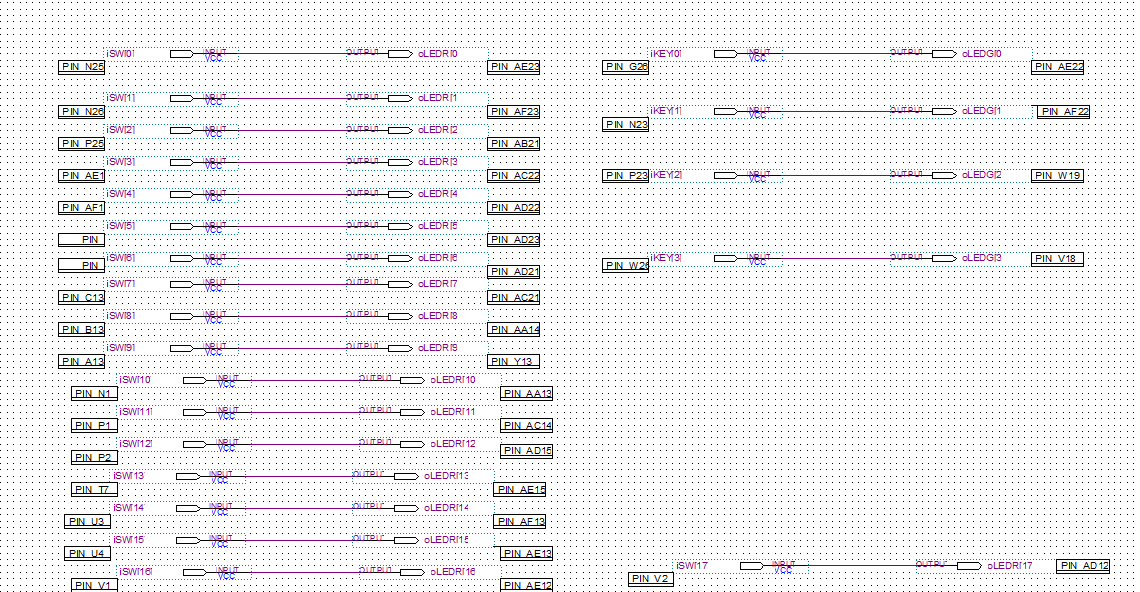
\includegraphics[width=15cm]{work1.PNG}
\end{center}
上の図のように回路を設計し、コンパイルし、FPGAに流し込んで動作させた。
\subsubsection{結果}
意図したとおりにトグルスイッチ(SW1 \textasciitilde SW17)と赤色LED(LEDR1 \textasciitilde LEDR17)、押しボタンスイッチ(KEY0 \textasciitilde KEY3)と緑色LED(LEDG0 \textasciitilde LEDG3)が対応して光ったり光らなかったりした。
\subsubsection{考察}
課題1では、単純な回路を設計して、主に設計、コンパイル、動作の流れを把握した。GUIで回路を設計するのは大変だと思った。
\subsection{課題2}
\subsubsection{目的}
押しボタンスイッチ(KEY0)を緑色LED(LEDG0,LEDG4)に、KEY1をLEDG1,LEDG5に、KEY2をLEDG2,LEDG6に、KEY3をLEDG3,LEDG7に接続した回路を作成し、動作させる。
\subsubsection{道のり}
\begin{center}
	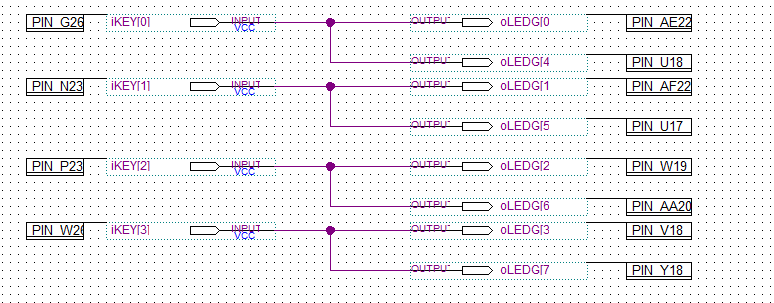
\includegraphics[width=15cm]{work2.PNG}
\end{center}
上の図のように回路を設計し、動作させた。
\subsubsection{結果}
意図したとおりに押しボタンスイッチ(KEY0)と緑色LED(LEDG0,LEDG4)が、KEY1とLEDG1,LEDG5が、KEY2とLEDG2,LEDG6が、KEY3とLEDG3,LEDG7が対応して光ったり、光らなかったりした。
\subsubsection{考察}
課題2では、配線を分岐させて、ひとつの入力と2つの出力をつなげるような回路を作成し、配線の分岐を作成する方法を習得した。
\subsection{課題3}
\subsubsection{目的}
課題1の回路と動作が反対(トグルスイッチを上げると赤色LEDが消灯し、押しボタンスイッチを押すと緑色LEDが消灯する。)に成るような回路を設計する。
\subsubsection{道のり}
\begin{center}
	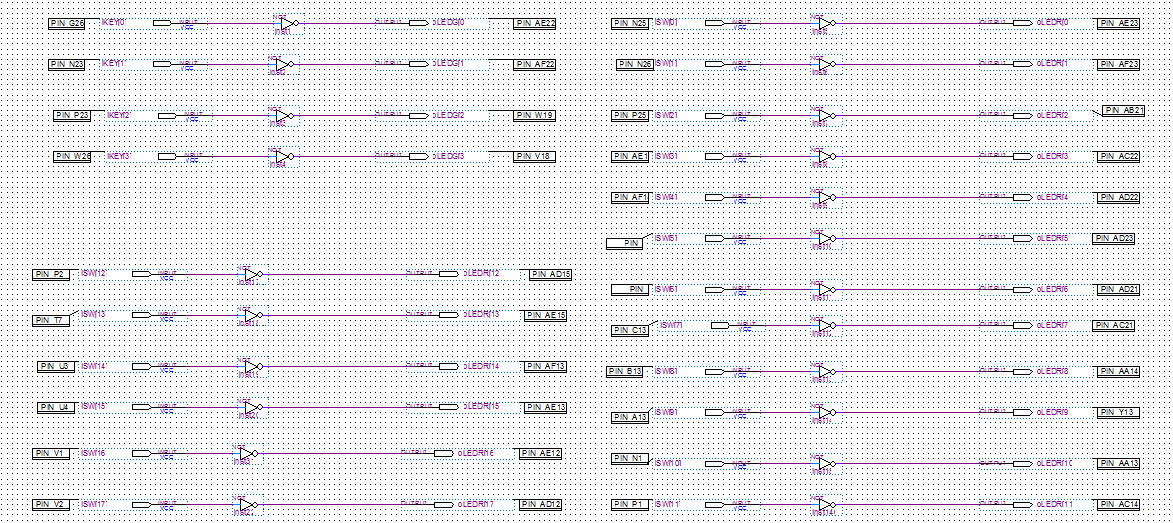
\includegraphics[width=15cm]{work3.PNG}
\end{center}
課題1のファイルをコピーペーストし、それを開いて上の図のように入力と出力の間にNOTゲートを挿入した。
\subsubsection{結果}
意図したとおりに課題1の回路と動作が反対(トグルスイッチを上げると赤色LEDが消灯し、押しボタンスイッチを押すと緑色LEDが消灯する。)に動作した。
\subsubsection{考察}
課題3では、課題1の回路を改造して課題1とは反対の動作をする回路を設計した。その過程でNOTゲートを使用し、回路上に基本的な論理ゲートを組み入れる方法を習得した。
\subsection{課題4}
\subsubsection{目的}
以下のように動作する回路を設計する。
\begin{itemize}
	\item SW0とSW1が両方とも1(上)であればLEDR0が点灯する回路(ANDゲート)
	\item SW2とSW3のうちひとつ以上が1であればLEDR2が点灯する回路(ORゲート)
	\item SW4とSW5のうち一方が1で他方が0であればLEDR4が点灯する回路(XORゲート)
\end{itemize}
\subsubsection{道のり}
\begin{center}
	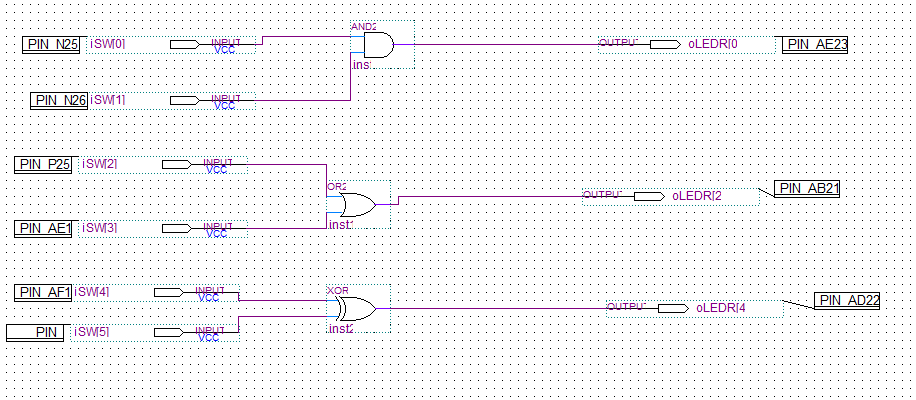
\includegraphics[width=15cm]{work4.PNG}
\end{center}
上の図のように回路を設計し、動作させた。
\subsubsection{結果}
%意図したとおりにSW0が1かつSW1が1のときLEDR0が光り、SW2が1またはSW3が1のときLEDR2が光り、SW4とSW5のうち一方が0で他方が1のときLEDR4が光った。
回路は正しく設計できていることが確認できたが、デバイス上では正しく動かなかった。
\subsubsection{考察}
課題4では6つのスイッチからの入力を2つずつAND、OR、XORにつなげ、その出力をそれぞれ別の赤色LEDに出力するような回路を設計した。その過程で、2つの入力を必要とする論理ゲートを回路に組み入れる方法を習得した。
\subsection{課題5}
\subsubsection{目的}
SW0からSW17のすべてを1にした時のみLEDR0が点灯する回路を設計する。
\subsubsection{道のり}
\begin{center}
	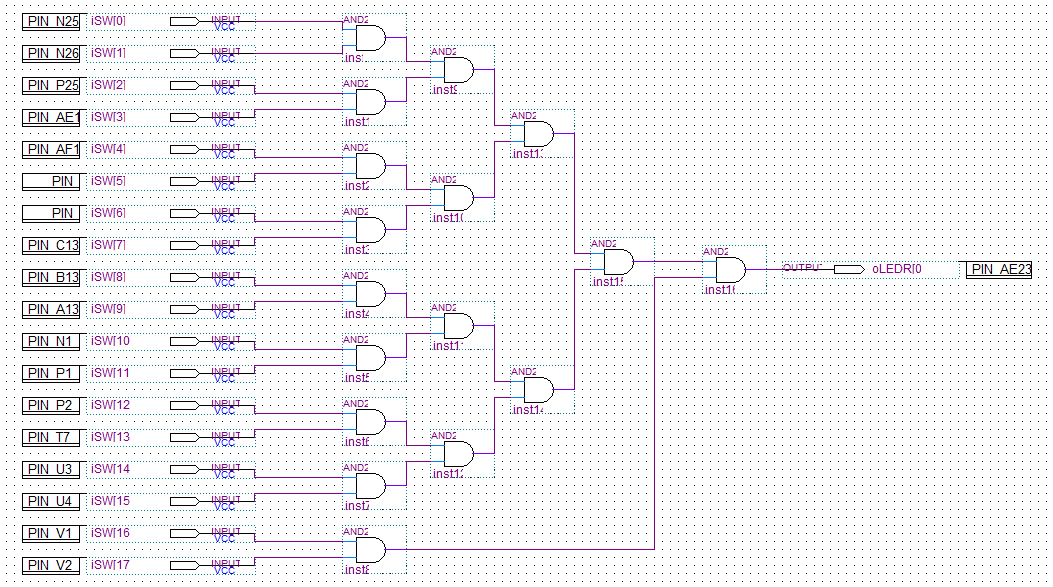
\includegraphics[width=15cm]{work5.PNG}
\end{center}
上の図のように複数のANDゲートを組み合わせて目的の回路を設計した。
\subsubsection{結果}
意図したとおりにSW0~SW17までのすべてのスイッチが1のときにのみLEDR0が点灯した。
\subsubsection{考察}
課題5では、多数のANDゲートを組み合わせてひとつの回路を設計した。それを通して、今までに学んだ様々な論理ゲートを用いてひとつの回路を設計することを体験した。GUIでの回路設計は、配線が意図しないようにつながってしまったりして効率的でないと感じた。
\subsection{課題6}
\subsubsection{目的}
NOT,AND,OR,XORゲートのみを用いて、1ビットの半加算器を作成し、それをmyhaと名づけて部品として定義し、myhaを用いて、入力AとBをトグルスイッチに、出力$C_{out}$とSをLEDにつないでテストする。
\subsubsection{道のり}
\begin{center}
	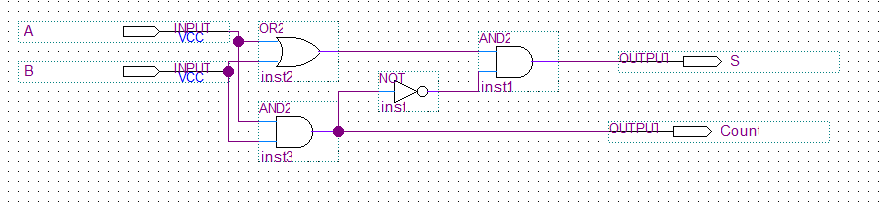
\includegraphics[width=15cm]{work6.PNG}
\end{center}
まず、上の図のような回路を設計し、これをmyhaと名づけて部品として定義した。
\begin{center}
	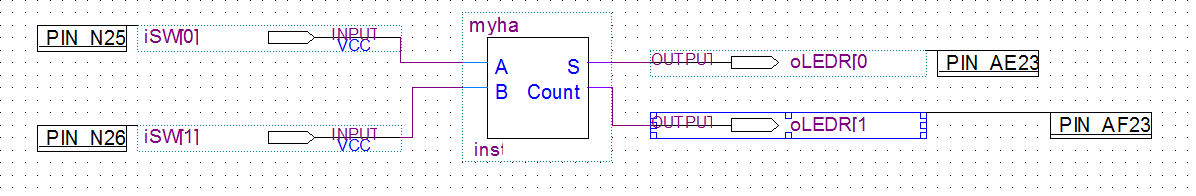
\includegraphics[width=15cm]{work6main.PNG}
\end{center}
次に、上の図のようにmyhaを配置して、入力と出力を対応するスイッチとLEDに接続した。
\subsubsection{結果}
教科書P258図5.1の半加算器の真理値表の通りに動作した。
\subsubsection{考察}
課題7では、NOT,AND,OR,XORゲートを用いて1ビットの半加算器を設計した。また、作成した回路をひとつの部品として定義し、再利用する方法を習得した。
\subsection{課題7}
\subsubsection{目的}
1ビットの全加算器を、次の2つの方法のいずれかを用いて設計し、入力AとBと$C_{in}$をトグルスイッチに、出力$C_{out}$とSをLEDにつないで、動作を確認する。
\begin{itemize}
	\item NOT,AND,OR,XORゲートのみを使って構成する。
	\item 半加算器を2つとORゲートを1つ使って構成する。
\end{itemize}
そして、半加算器の場合と同様に、構造化設計を用いて作成した全加算器をmyfaと名づけて定義し、トップレベルの回路図に貼り付けてテストする。
\subsubsection{道のり}
\begin{center}
	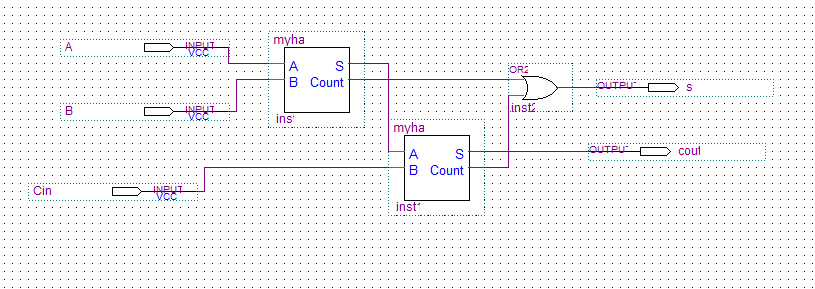
\includegraphics[width=15cm]{work7myfa.PNG}
\end{center}
今回は後者の半加算器を2つとORゲートを1つ使って構成する方法を取り、上の図のように全加算器を設計した。
\begin{center}
	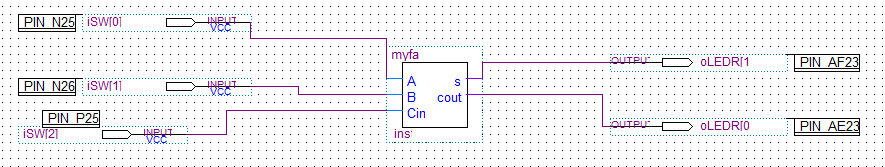
\includegraphics[width=15cm]{work7main.PNG}
\end{center}
その後、課題6の半加算器の場合と同様に、作成した全加算器をmyfaと名づけて定義し、上の図のように入力をスイッチに、出力をLEDに接続した。
\subsubsection{結果}
教科書P258図5.3の全加算器の真理値表の通りに動作した。
\subsubsection{考察}
課題6の全加算器の場合と同様に、全加算器を作成して一つの部品として定義し、動作を確認することができた。構造化設計を用いて、ある程度複雑な回路も比較的効率的に設計することができると思った。
\subsection{課題8}
\subsubsection{目的}
2:4デコーダを設計し、入力と出力に適宜スイッチやLEDをつないで動作を確認する。
\subsubsection{道のり}
\begin{center}
	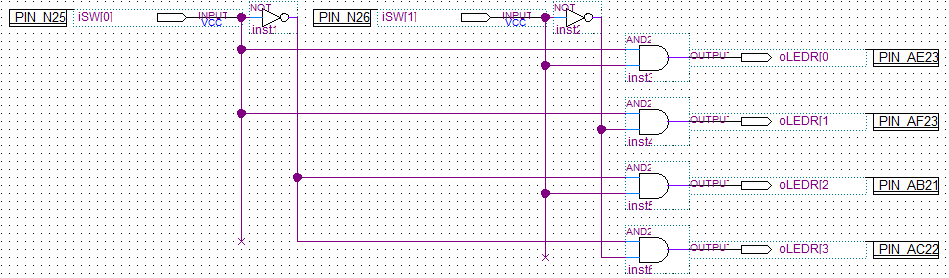
\includegraphics[width=15cm]{work8.PNG}
\end{center}
上の図のように回路を設計し、動作させた。
\subsubsection{結果}
教科書P89図2.63の2:4デコーダの真理地表のとおりに動作した。
\subsubsection{考察}
課題8では基本的な論理ゲートを用いて2:4デコーダを作成した。それ以前の課題に比べて回路が複雑だったので、配線の接続や重なりに注意して作成する必要があった。
\subsection{課題9}
\subsubsection{目的}
3:8デコーダを設計し、入力と出力に適宜スイッチやLEDをつないで動作を確認する。
\subsubsection{道のり}
\begin{center}
	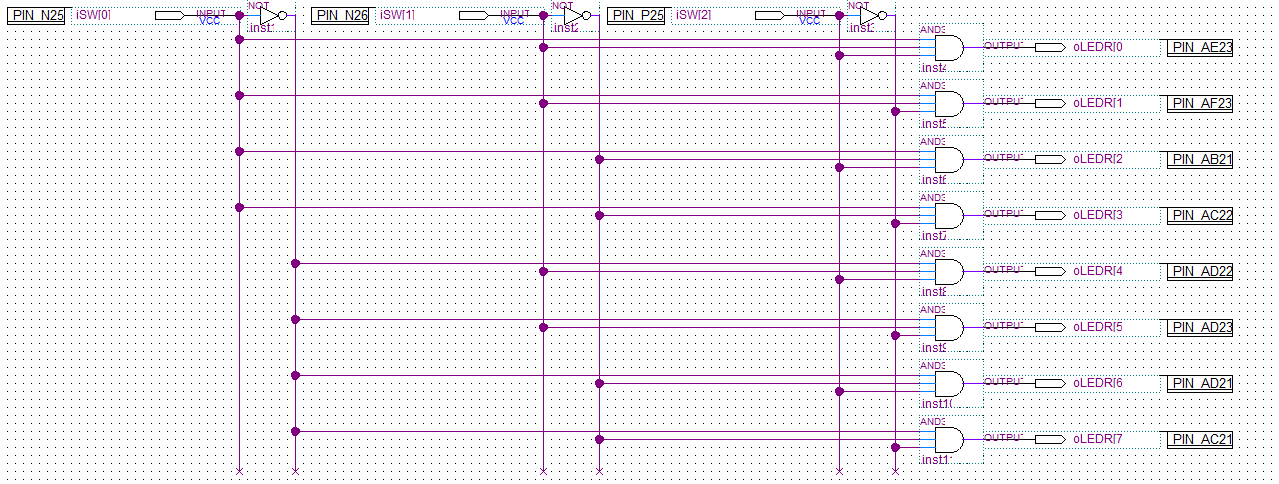
\includegraphics[width=15cm]{work9.PNG}
\end{center}
上の図のように回路を設計し、動作させた。
\subsubsection{結果}
入力のSW0,SW1,SW2の値を並べた2進数をnとした時、LEDRnが光った。
\subsubsection{考察}
課題9では、課題8と構造はほぼ同じだが、より大きく、複雑な回路を設計することになったので、回路の作成はより面倒な作業になった。
\subsection{課題10}
\subsubsection{目的}
2:1マルチプレクサを設計し、入力と出力に適宜スイッチやLEDをつないで動作させる。
\subsubsection{道のり}
\begin{center}
	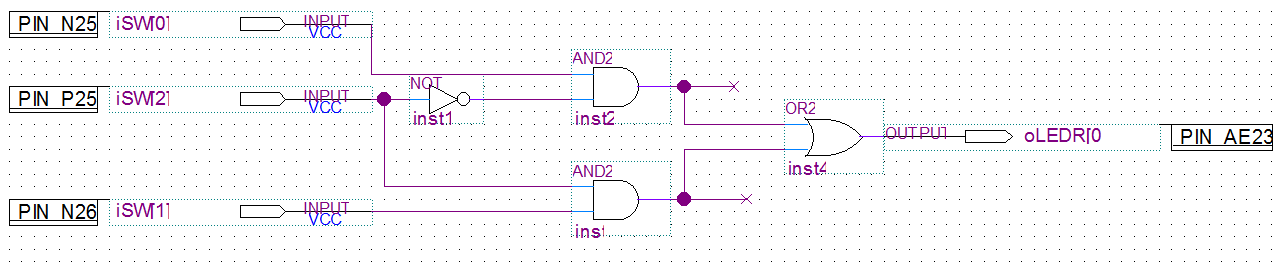
\includegraphics[width=15cm]{work10.PNG}
\end{center}
上の図のようにSW2が0であればSW0の値がLEDR0に出力され、SW2が1であればSW1の値がLEDR0に出力されるように回路を設計し、動作させた。
\subsubsection{結果}
意図したとおりに、SW2が0であればSW0の値がLEDR0に出力され、SW2が1であればSW1の値がLEDR0に出力された。教科書P85図2.54の$D_0$がSW0に、$D_1$がSW1に、SがSW2に、YがLEDR0に対応している。
\subsubsection{考察}
課題10では、2:1マルチプレクサをAND,NOTゲートを用いて作成した。この問題を解決したことによって、複数の入力から一つの値を選び出力するマルチプレクサの原理を理解することが出来た。
\subsection{課題11}
\subsubsection{目的}
4:1マルチプレクサを設計し、入力と出力を適宜スイッチやLEDをつないで確認する。
\subsubsection{道のり}
\begin{center}
	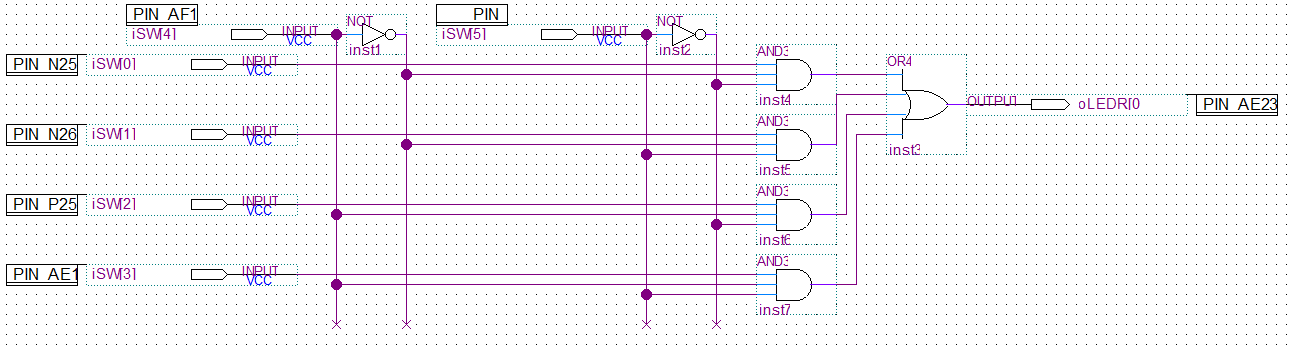
\includegraphics[width=15cm]{work11.PNG}
\end{center}
上の図のように、SW4,SW5の値がそれぞれ00のときはSW0が、01のときはSW1が、10のときはSW2が、11のときはSW3がLEDR0として出力されるように回路を設計し、動作させた。
\subsubsection{結果}
意図したとおりに、SW4,SW5の値がそれぞれ00のときはSW0が、01のときはSW1が、10のときはSW2が、11のときはSW3がLEDR0として出力された。教科書P86図2.57の$D_0$がSW0に、$D_1$がSW1に、$D_2$がSW2に、$D_3$がSW3に、$S_{1:0}$がSW4とSW5に、YがLEDR0に対応している。
\subsubsection{考察}
課題10で作成した2:1マルチプレクサを拡張して、4:1マルチプレクサを作成した。2:1マルチプレクサも、4:1マルチプレクサも原理的には同じで、入力、配線、ゲートの個数が異なるだけであることが分かったが、回路がより複雑になり、GUIでの回路の作成が困難になることも分かった。
\subsection{課題12}
\subsubsection{目的}
表\ref{Report12TruthTable}に示す真理値表のような3入力の多数決回路を設計し、動作を確認する。
%\begin{comment}
\begin{table}[ht]
	\begin{center}
		\caption{入力多数決回路の真理値表}
		\label{Report12TruthTable}
		\begin{tabular}{|c|c|c||c|}		\hline
			A0	&A1	&A2	&Y\\	\hline\hline
			0	&0	&0	&0\\	\hline
			0	&0	&1	&0\\	\hline
			0	&1	&0	&0\\	\hline
			0	&1	&1	&1\\	\hline
			1	&0	&0	&0\\	\hline
			1	&0	&1	&1\\	\hline
			1	&1	&0	&1\\	\hline
			1	&1	&1	&1\\	\hline
		\end{tabular}
	\end{center}
\end{table}
%\end{comment}
\subsubsection{道のり}
表\ref{Report12TruthTable}の真理値表をもとに表\ref{Report12KarnaughMap}に示しているカルノー図を書き、出力Yは入力A0,A1,A2を使って$Y=A0 \cdot A1+A1 \cdot A2 + A2 \cdot A0$と表されることがわかった。
%\begin{comment}
\begin{table}[ht]
	\begin{center}
		\caption{入力多数決回路のカルノー図}
		\label{Report12KarnaughMap}
		\begin{tabular}{|c||c|c|}				\hline
			\backslashbox{A1,A0}{A2}	&0	&1\\	\hline\hline
			00				&0	&0\\	\hline
			01				&0	&1\\	\hline
			11				&1	&1\\	\hline
			10				&0	&1\\	\hline
		\end{tabular}
	\end{center}
\end{table}
%\end{comment}
\begin{center}
	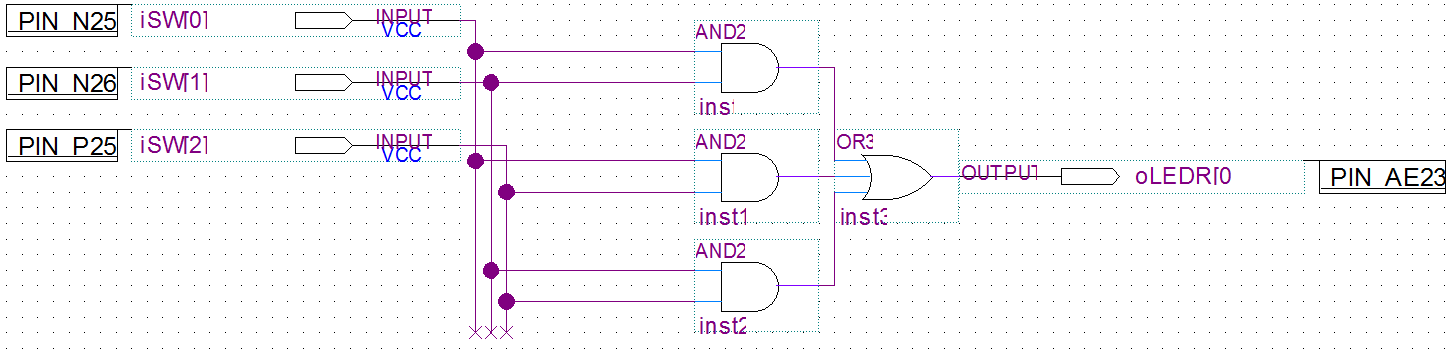
\includegraphics[width=15cm]{work12.PNG}
\end{center}
次に、表\ref{Report12KarnaughMap}のカルノー図によって導き出した論理式に基いて、上の図のような回路を作成し実行した。
\subsubsection{結果}
意図したとおりに、入力A0.A1,A2の多数決によって出力Yが決まるように動作した。
\subsubsection{考察}
課題12では、入力多数決回路の真理値表からカルノー図を書いて論理式を導き出し、回路を作成することができた。今回は真理値表やカルノー図も小さく、回路もそれほど複雑ではなかったため、比較的容易に設計し、理解することができた。
\section{実験の総括的なまとめ・感想}
今回はソフトウェアのプログラミングというよりもGUI上で視覚的に回路を設計し実際に動作させるというものだった。GUI上でも回路の設計は比較的単純な回路の場合には設計・作成も簡単で、作成したあともひと目で見てそれがどのような回路かわかったが、複雑な回路では配線が複雑に重なりあい回路の作成中に配線が意図しないとろこに接続されてしまうこともあり、回路が完成してもとても見づらい回路になってしまった。また今回はLaTeXを用いてレポートを作成し画像や表の作り方などの基本的な機能を習得した。
\end{document}
